\section{Experiments}
\begin{frame}{Experiments}
\begin{figure}
    \centering
    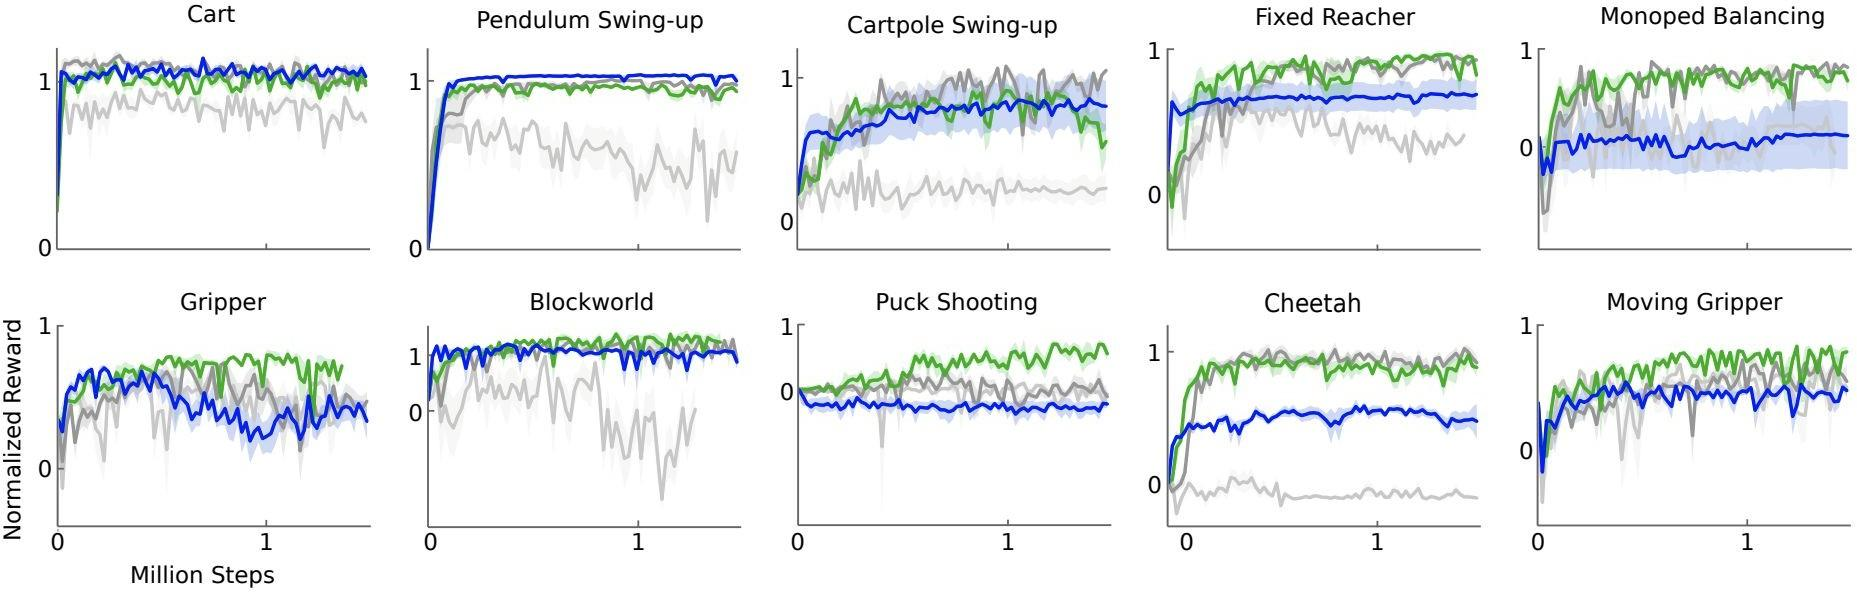
\includegraphics[width=0.95\textwidth,height=0.55\textheight,keepaspectratio]{images/continuous-control-1/figures/experiments-target-batchnorm.jpg}
\end{figure}
\begin{itemize}
    \footnotesize
    \item[] \textcolor{gray}{Light Grey:} Original DPG
    \item[] \textcolor{black!60}{Dark Grey:} Target Network
    \item[] \textcolor{green!60!black}{Green:} Target Network + Batch Norm
    \item[] \textcolor{blue}{Blue:} Target Network from pixel-only
\end{itemize}
\begin{flushright}\tiny Figure: DDPG \rref{5}\end{flushright}
\end{frame}

\begin{frame}{Experiments}
\vspace{-0.5em}
\begin{center}
\textcolor{red}{Do target networks and batch norm matter?}
\end{center}
\begin{figure}
    \centering
    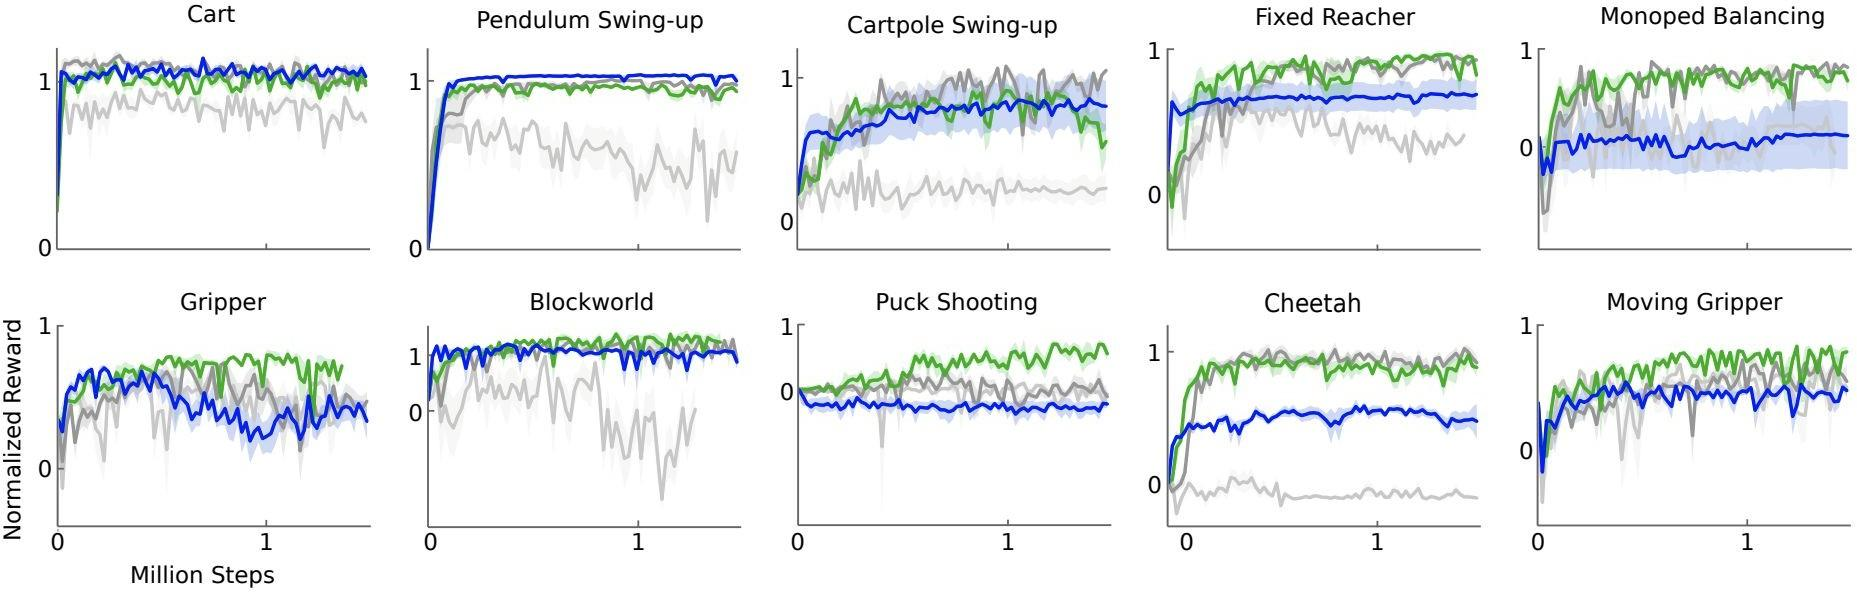
\includegraphics[width=0.95\textwidth,height=0.5\textheight,keepaspectratio]{images/continuous-control-1/figures/experiments-target-batchnorm.jpg}
\end{figure}
\begin{itemize}
    \footnotesize
    \item[] \textcolor{gray}{Light Grey:} Original DPG
    \item[] \textcolor{black!60}{Dark Grey:} Target Network
    \item[] \textcolor{green!60!black}{Green:} Target Network + Batch Norm
    \item[] \textcolor{blue}{Blue:} Target Network from pixel-only
\end{itemize}
\begin{flushright}\tiny Figure: DDPG \rref{5}\end{flushright}
\end{frame}
